\section*{Results}
\subsection*{Maximizing decrease key calls}
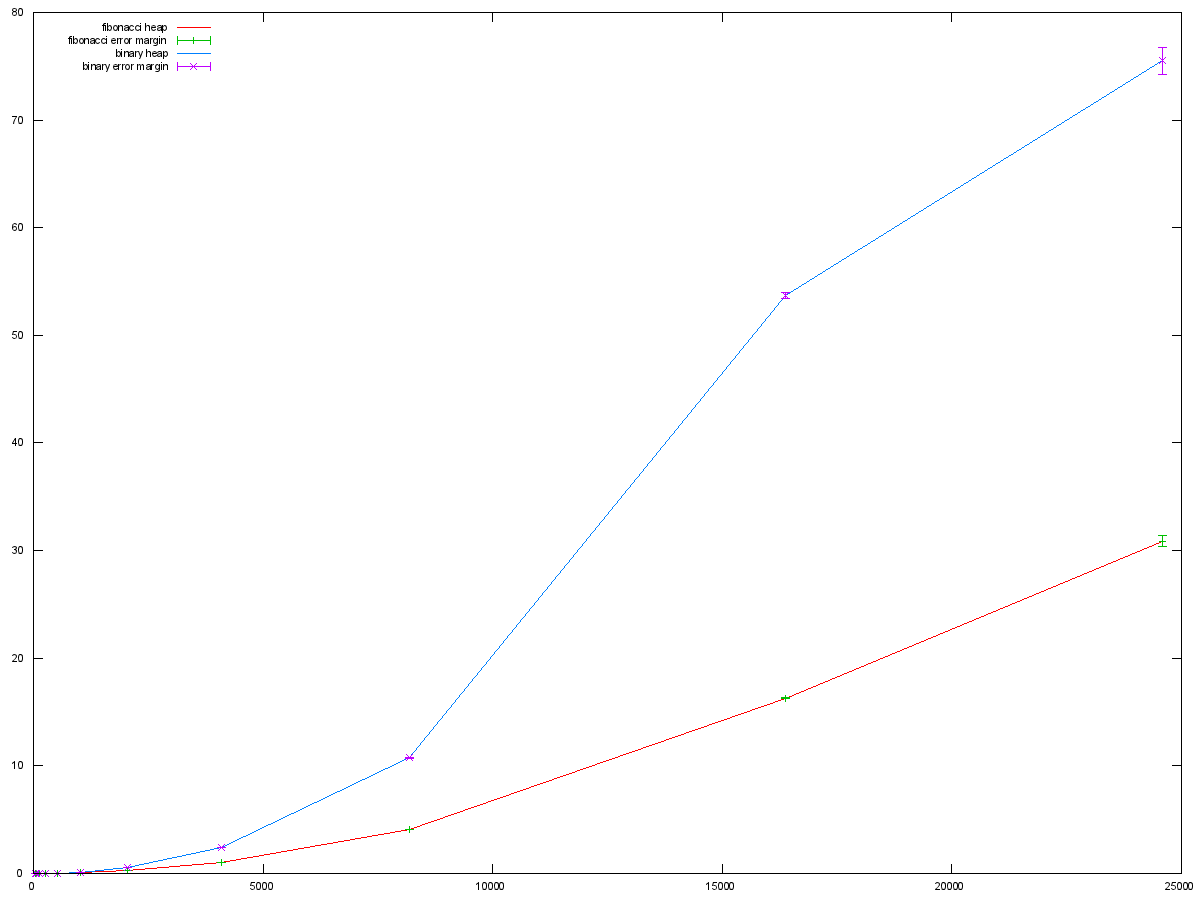
\includegraphics[scale=0.30]{../results/fibonacci-binary-dkmax2.png}
 
It's rather obvious that Binary Heap performs significantly worse than Fibonacci Heap, just as expected. The Binary Heap curve has an odd shape, but we triple checked the results, so our guess is that some underlying VM or hardware played a role, most likely page faults.
\subsection*{Random Graphs}
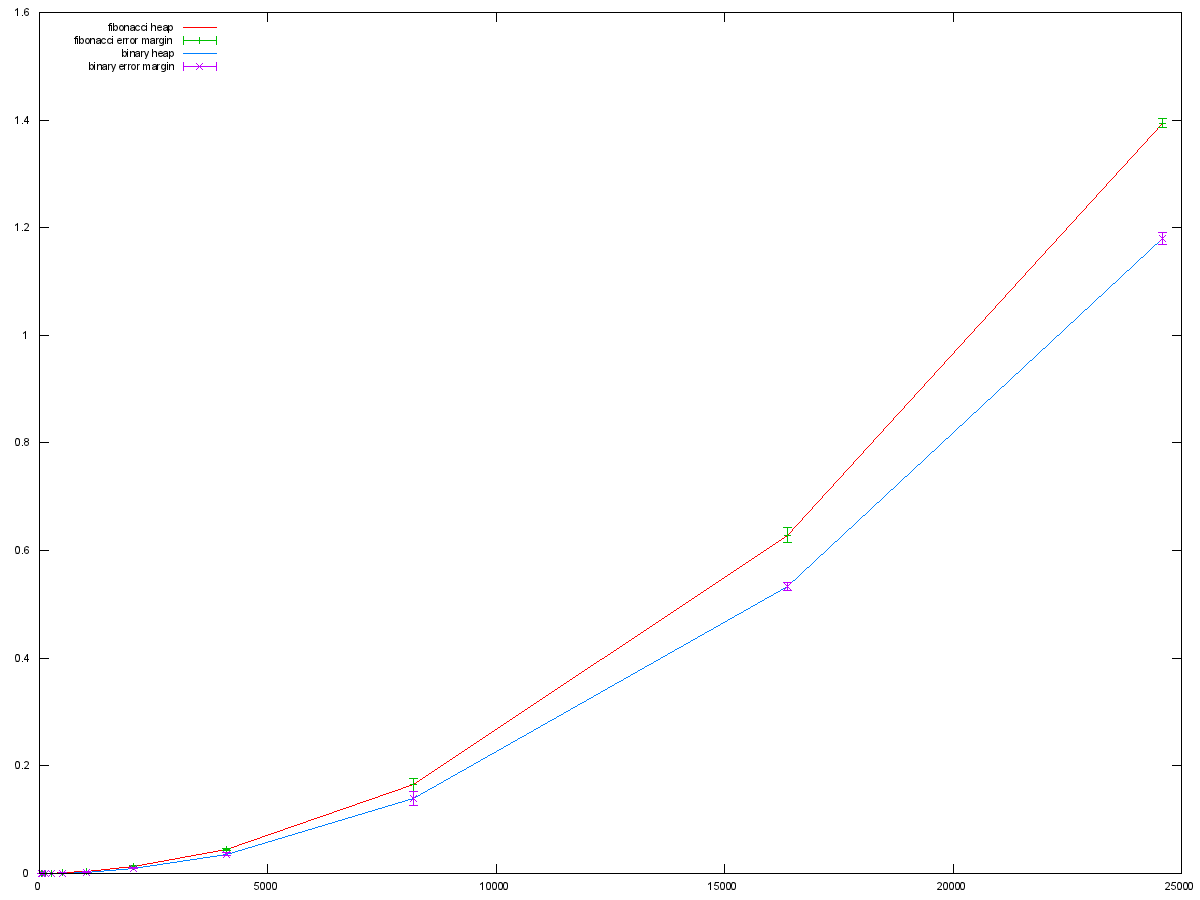
\includegraphics[scale=0.30]{../results/fibonacci-binary-random.png}

Here we see that the difference between Binary and Fibonacci heaps are almost insignificant, but with Binary Heap leading. The graphs was created with chance of edge 15\% and max weight 20.
\section*{Conclusion}
It's fairly obvious that unless given a graph, that is constructed in such a way that maximize \textit{decrease key} calls and the work the Binary Heap have to do, then then Binary Heap is to be prefered due to the much smaller constants.